\documentclass[aspectratio=1610, dvipsnames, xcolor=table]{beamer}

\setbeamersize{text margin left=3mm,text margin right=3mm} 
\usepackage{t1enc}
\usepackage[magyar]{babel}
\usepackage{subcaption}
\usepackage[export]{adjustbox}
\usepackage[table]{xcolor}



\definecolor{szin1}{rgb}{0.5, 0.188, 0.478}
\definecolor{szin2}{RGB}{196, 203, 133}
\definecolor{szin3}{cmyk}{0, 0.7771, 0.5437, 0.8656}
\definecolor{szin4}{gray}{0.5}

\usepackage{graphics}
\usepackage{wrapfig}

\usetheme{Malmoe}
\usecolortheme{crane}

\title{Féléves beadandó}
\author{Nagy Róbert és Bartók-Balogh Gábor}
\date{\today}
\subtitle{Prezentáció  \LaTeX-kel az \textbf{xcolor} csomagról}
\institute{Miskolci Egyetem}


\begin{document}
 % titleslide
    \frame[plain]{\maketitle}

        
        % slide 1 
    \begin{frame}[fragile]{Az xcolor csomag alapjai}
        \begin{minipage}{0.6\textwidth}
            \begin{itemize}
            \item \onslide<1->\verb!\usepackage[<Opciók>]{xcolor}!
            \item \onslide<2->Az xcolor lehetővé teszi, hogy kiszínezzünk szöveget,táblázatot, rajzolt ábrákat, stb... 
            \item \onslide<3->Használhatunk névvel ellátott színeket
            \item \onslide<4->Alapból 19 darab van.
            \item \onslide<5->dvipsnames opcióval 68 darab
            \item \onslide<5->svgnames opcióval 151 darab 
            \item \onslide<5->x11names opcióval pedig 317 darab
            \end{itemize}
        \end{minipage} \hfill
        \begin{minipage}{0.35\textwidth}    
            \begin{figure}
                \onslide<4->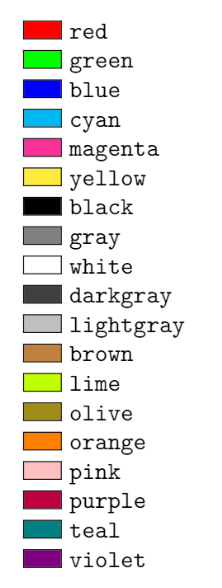
\includegraphics[scale=0.4]{img/szinek.png}
                \onslide<4->\caption{Névvel ellátott színek}
            \end{figure}
        \end{minipage}
    \end{frame}

    % slide 2
    \begin{frame}[fragile]{Az xcolor csomag alapjai}
        \begin{minipage}{0.8\textwidth}
            \begin{itemize}
                \item \onslide<1->Definiálhatunk saját színeket is.
                \item \onslide<2->\verb!\definecolor{<név>}{<Mód>}{<Értékek>}!
                \item \onslide<3->A mód lehet
                \begin{enumerate}
                    \item \onslide<4->rgb
                    \item \onslide<4->RGB
                    \item \onslide<4->cmyk
                    \item \onslide<4->gray    
                \end{enumerate}
                Például:
                \item \onslide<5->\verb!\definecolor{szin1}{rgb}{0.500, 0.188, 0.478}! \hfill \textcolor{szin1}{Szín1}
                \item \onslide<5->\verb!\definecolor{szin2}{RGB}{196, 203, 133}! \hfill \textcolor{szin2}{Szín2}
                \item \onslide<5->\verb!\definecolor{szin3}{cmyk}{0, 0.7771, 0.5437, 0.8656}! \hfill \textcolor{szin3}{Szín3}
                \item \onslide<5->\verb!\definecolor{szin4}{gray}{0.5}! \hfill \textcolor{szin4}{Szín4}
            \end{itemize}                                                        
        \end{minipage} 
    \end{frame}
    
    %slide 3
    \begin{frame}[fragile]{color használata}
        \begin{minipage}{0.6\textwidth}
            \begin{itemize}            
                \item \onslide<1-> színek használata: \verb!\color{<szín>}!
                \item \onslide<2-> lehet használni: szövegnél, listáknál stb...    
            \end{itemize}
        \end{minipage}
        \begin{minipage}{0.35\textwidth}
            
                \onslide<1-> például:
                \onslide<1-> \begin{verbatim}\begin{itemize}
    \color{Aquamarine}
    \item első
    \item második
\end{itemize}\end{verbatim}
                 \onslide<2-> \begin{itemize}
                    \color{Aquamarine}
                    \item első
                    \item második
                \end{itemize}
        \end{minipage}
    \end{frame}
       
    %slide 4
    \begin{frame}[fragile]{szöveg szín és háttér beállítása}
        
        \begin{itemize}            
            \item \onslide<1-> szövegszín beállítása: \verb!\textcolor{<szín>}{<szöveg>}!
            \item \onslide<1-> például: \verb!\textcolor{brown}{szöveg van itt}! = \textcolor{brown}{szöveg van itt}
            \item \onslide<2-> szövegháttér beállítása: \verb!\colorbox{<szín>}{<szöveg>}!
            \item \onslide<2-> például: \verb!\colorbox{yellow}{szöveg}! = \colorbox{yellow}{szöveg}
            \item \onslide<3-> szövegháttér + keret beállítása: \verb!\fcolorbox{<keret szine>}{<háttér szine>}{<szöveg>}!
            \item \onslide<3-> például: \verb!\fcolorbox{black}{yellow}{szöveg}! = \fcolorbox{black}{yellow}{szöveg}
            \item \onslide<4-> Az egész oldal kiszinezése: \verb!\pagecolor{<szín>}!
        \end{itemize}
    \end{frame}
    

    % slide 5
    \begin{frame}[fragile]{Táblázat színezés}
        \begin{center}
            A \verb!\usepackage[table]{xcolor}! package implementálása után tudunk táblázatban is hasonló dolgokat alkotni.
            \noindent
            {\color{Dandelion} \rule{\linewidth}{1mm}}
        \end{center}

        \vfill
        \begin{center}
            \onslide<2->\begin{tabular}{|c|c|c|}
                \hline
                \rowcolor{Apricot}Helyezés & Versenyző & Idő \\
                \cellcolor{ForestGreen}1 & \cellcolor{Orchid}Ákos & \cellcolor{Aquamarine}1:11:210 \\
                \cellcolor{Yellow}2  & \cellcolor{Mulberry}András & \cellcolor{Emerald}1:22:156  \\
                \cellcolor{BurntOrange}3 & \cellcolor{Plum}Tomi  &  \cellcolor{PineGreen}1:30:155 \\
                \hline
            \end{tabular}
        \end{center}
    \end{frame}

    % slide 6
    \begin{frame}[fragile]{Táblázat színezés}
        \onslide<1->\begin{block}{Instukció}
            A \verb!\usepackage[table]{xcolor}! implementálás után a documentclassban meg kell adnunk a következő sort:\textbf{"xcolor=table"}
        \end{block} 
        \onslide<2->\begin{exampleblock}{Példa}
        {
            \verb!\documentclass[dvipsnames,xcolor=table]{beamer}!
            \verb!\usepackage[table]{xcolor}!
        }
        \end{exampleblock}	
        \begin{figure}[H]
            \onslide<2->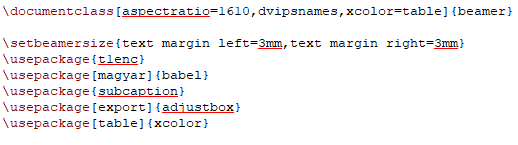
\includegraphics[scale=0.8]{img/tablesetup.png}
            \onslide<2->\caption{Felállítás}
        \end{figure}
    \end{frame}

    % slide 7
    \begin{frame}[fragile]{Táblázat színezés}
    \begin{center}
        \LaTeX-ben való alkalmazás
        \noindent
        {\color{Dandelion} \rule{\linewidth}{1mm}}
    \end{center}
        \begin{figure}[H]
            \onslide<2->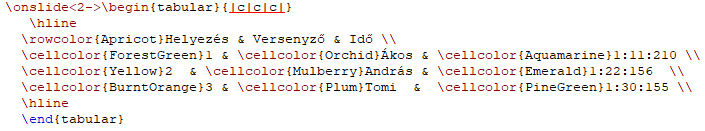
\includegraphics[scale=0.8]{img/tablealkalmazas.png}        
        \end{figure}
    \end{frame}

    

    % slide 8
    \colorlet{mygreen}{green!40!yellow}
    \colorlet{mygreencomp}{-green!40!yellow} 

    \begin{frame}[fragile]{Színek keverése}
        \begin{itemize}
            \item \onslide<1->Keveréssel létrehozott színek mentése: \verb!\colorlet{<új szín neve>}{<keverés>}!
            \item \onslide<2->keverés kifejezés részei: $$<\text{százalék}>_1!<\text{szín}>_1!<\text{százalék}>_2!\ldots!<\text{százalék}>_n!<\text{szín}>_n$$
            \item \onslide<2->például: \begin{verbatim}\colorlet{mygreen}{green!40!yellow}\end{verbatim} 
            \item \onslide<3->40\% zöld 60\% sárgával keverve \fcolorbox{black}{mygreen}{ } 
            \item \onslide<4->Komplementere: \fcolorbox{black}{mygreencomp}{ } \begin{verbatim}\colorlet{mygreen}{-green!40!yellow}\end{verbatim} 
            


        \end{itemize}
    \end{frame}
    % slide 12
    \begin{frame}{Vége}
        
        \centering \Huge Köszönjük a figyelmet!
        
    \end{frame}
\end{document}